% =============================================================================
%  CS375 A9 - Address Translation: Lab Report
%  Build:  cd report && pdflatex report.tex && pdflatex report.tex
%     or:  make report     (from the repository root; copies PDF to submission/)
%
%  Screenshots: save PNGs into report/screenshots/ using the names listed in
%  report/screenshots/README.md. Missing screenshots show a placeholder box.
% =============================================================================
\documentclass[11pt]{article}

\usepackage[margin=1in]{geometry}
\usepackage[T1]{fontenc}
\usepackage{lmodern}
\usepackage{amsmath}
\usepackage{graphicx}
\usepackage{float}
\usepackage{caption}
\usepackage{booktabs}
\usepackage{xcolor}
\usepackage{listings}
\usepackage{enumitem}
\usepackage{fancyhdr}
\usepackage[hidelinks]{hyperref}

% ---------------------------------------------------------------- fill me in
\newcommand{\studentname}{Your Name}
\newcommand{\coursename}{CS375 -- Operating Systems}
\newcommand{\assignment}{A9 -- Address Translation}

% Set to \includecodetrue to append the full source listing to the report.
\newif\ifincludecode
\includecodefalse

% ---------------------------------------------------------------- helpers
\graphicspath{{screenshots/}}

% \screenshot[graphics options]{file.png}{caption}{label}
% Screenshots are 144 dpi, so in trim={left bottom right top} 1 px = 0.5 bp.
\newcommand{\screenshot}[4][width=\linewidth,height=0.55\textheight,keepaspectratio]{%
  \begin{figure}[H]
    \centering
    \IfFileExists{screenshots/#2}{%
      \includegraphics[#1]{#2}%
    }{%
      \fbox{\parbox[c][3.5cm][c]{0.9\linewidth}{\centering
        \textbf{Screenshot not added yet}\\[4pt]
        save it as \texttt{report/screenshots/\detokenize{#2}}}}%
    }
    \caption{#3}
    \label{#4}
  \end{figure}}

\lstset{
  basicstyle=\ttfamily\footnotesize,
  columns=fullflexible,
  keepspaces=true,
  breaklines=true,
  frame=single,
  backgroundcolor=\color{gray!6},
  rulecolor=\color{gray!40},
  numbers=left,
  numberstyle=\tiny\color{gray},
  keywordstyle=\color{blue!70!black}\bfseries,
  commentstyle=\color{green!40!black},
  stringstyle=\color{red!60!black},
}
\lstdefinestyle{term}{numbers=none,language={},backgroundcolor=\color{gray!4}}

\newcommand{\code}[1]{\texttt{\detokenize{#1}}}
\newcommand{\question}[1]{\par\medskip\noindent\textbf{#1}\par\smallskip}

\setlength{\headheight}{14pt}
\pagestyle{fancy}
\fancyhf{}
\lhead{\coursename}
\rhead{\assignment}
\cfoot{\thepage}

\setlist{itemsep=2pt,topsep=4pt}
\setlength{\emergencystretch}{3em}

% =============================================================================
\begin{document}

\begin{titlepage}
  \centering
  \vspace*{3cm}
  {\Huge\bfseries Advanced Segmented, Paged\\[6pt] Memory Model Simulator\par}
  \vspace{1cm}
  {\Large Lab Report -- \assignment\par}
  \vspace{2cm}
  {\large \studentname\par}
  \vspace{0.3cm}
  {\large \coursename\par}
  \vspace{0.3cm}
  {\large \today\par}
  \vfill
  {\small Source: \code{memory_simulator.cpp} \quad Build: \code{g++ -std=c++17 -O2 -o memory_simulator memory_simulator.cpp}\par}
\end{titlepage}

\tableofcontents
\newpage

% =============================================================================
\section{Overview}

The simulator models a virtual memory system that combines segmentation with
two-level paging. A logical address is the tuple
\[
  (\textit{segment},\ \textit{directory index},\ \textit{page},\ \textit{offset},\ \textit{access})
\]
and translates to a physical address
\[
  \textit{physical} = \textit{frame} \times \textit{page\_size} + \textit{offset}.
\]
Each segment has a \emph{base address} (the location of its page directory), a
\emph{limit} in pages and a protection mode (read-only or read-write). The segment's page
directory (\code{DirectoryTable}) points to second-level page tables (\code{PageTable}).
These are created only when a region is first used. Every page-table entry holds a frame number,
a present bit, its own protection and a last-access time. A fixed-size
\code{PhysicalMemory} pool tracks which page owns each frame and supports FIFO and LRU
replacement.

\subsection{Implemented features}
\begin{center}\small
\begin{tabular}{@{}lp{0.68\linewidth}@{}}
\toprule
Requirement & Implementation \\
\midrule
Protection enforcement & segment \emph{and} page RO/RW checks; access type R/W in all inputs \\
Page replacement & FIFO (load-order queue) and LRU (per-frame last use), switchable at runtime \\
Multi-level paging & \code{DirectoryTable} $\rightarrow$ lazily allocated \code{PageTable}s \\
Dynamic configuration & prompts with defaults/validation, config file, \emph{Reconfigure} menu item \\
Stress testing & $N$ random addresses with a configurable valid ratio $\rightarrow$ \code{results.txt} \\
Utilization tracking & frames used / total, reported after every batch \\
Batch processing & addresses from a file, per-line results and summary \\
Simulated latency & 1--5 units per translation, +10 for a serviced page fault, history across runs \\
Error logging & detailed reasons (e.g.\ ``Invalid segment 5, max 2'') in \code{errors.log} \\
Visualization & memory map (segments, directories, pages, frame map) and Gantt timeline \\
Experiments & FIFO vs LRU on three workloads; page size 1000 vs 4000 \\
\bottomrule
\end{tabular}
\end{center}

\subsection{Translation algorithm}
\begin{enumerate}
  \item Look up the segment. If it does not exist $\Rightarrow$ \emph{segmentation fault}.
  \item Check the directory index, the page number (against the segment limit) and the
        offset (against the page size) $\Rightarrow$ \emph{directory fault}, \emph{limit violation},
        \emph{offset fault}.
  \item Write to a read-only segment $\Rightarrow$ \emph{protection violation}.
  \item If the directory entry is empty, allocate a page table for it.
  \item Write to a read-only page $\Rightarrow$ \emph{protection violation}. If the present bit is 0
        $\Rightarrow$ \emph{page fault}: use a free frame, or else evict the FIFO/LRU victim
        and clear the victim's present bit.
  \item Compute the physical address and update LRU/FIFO bookkeeping and metrics.
\end{enumerate}

\subsection{Corrections to the starter code}
\begin{itemize}
  \item The starter computed \code{base + frame * page_size + offset}. Frames already have
        absolute positions, so adding the segment base relocated twice and made segments
        overlap (segment~0 frame~12 = segment~1 frame~2). The simulator uses
        \code{frame * page_size + offset}. The base locates the page directory.
  \item The starter's fault handler called \code{setFrame(page, frame, accessType)}. A write
        to a non-present read-only page therefore \emph{upgraded} that page to read-write. Protection is
        now a fixed attribute of the page and is checked before any fault is serviced.
  \item The starter gave initial pages \texttt{rand() \% 100} as frame numbers, ignoring the frame
        pool (pages could alias or point past physical memory). Initial pages now claim
        real free frames with recorded owners, so eviction can update the right page table.
\end{itemize}

% =============================================================================
\section{Test Configuration}

All screenshots use \code{sample_config.txt} with seed 42, so the runs are reproducible:

\begin{lstlisting}[style=term]
frames 7
page_size 1000
pages_per_dir 4
policy LRU
0  0x1000  6   RO   2:RO 5:RO -:RO -:RO             # code
1  0x2000  8   RW   0:RW -:RW 6:RW -:RO 3:RW -:RW    # data
2  0x3000  12  RW   1:RW -:RW                       # stack
\end{lstlisting}

This gives 26 virtual pages over 7 frames (3.71$\times$ over-committed). Six pages are resident at
start, and one frame (4) is free. Segment~0 directory~1 and segment~2 directories~1--2 start
unallocated.

\screenshot{00_build.png}{Building the simulator with \code{-Wall -Wextra} (no warnings).}{fig:build}

% =============================================================================
\section{Results}

\subsection{Manual translations}
Five manual translations mixing valid and invalid addresses:

\begin{center}\small
\begin{tabular}{@{}clp{0.62\linewidth}c@{}}
\toprule
\# & Logical address & Outcome & Latency \\
\midrule
1 & (1,0,2,250,R) & hit in frame 6 $\rightarrow$ physical 6250 & 3 \\
2 & (0,0,1,999,W) & protection violation (segment 0 is read-only) & 3 \\
3 & (2,1,2,40,W) & directory allocated, page fault $\rightarrow$ free frame 4 $\rightarrow$ 4040 & 12 \\
4 & (5,0,0,0,R) & segmentation fault: invalid segment 5, max 2 & 5 \\
5 & (1,1,3,100,R) & page fault, memory full, LRU evicts S1:D0:P0 from frame 0 $\rightarrow$ 100 & 12 \\
\bottomrule
\end{tabular}
\end{center}

\screenshot[height=0.78\textheight,keepaspectratio,trim={0 0 565 11},clip]{01_manual_translations.png}{Sample run: five manual address translations (valid and invalid).}{fig:manual}
\screenshot[height=0.78\textheight,keepaspectratio,trim={0 0 464 23},clip]{02_memory_map.png}{Memory map after the five translations: segment table, directories,
page tables and frame ownership.}{fig:map}

\subsection{Random address stress test}
100 random addresses with a valid ratio of 0.70 (72 in range, 28 out of range):

\begin{center}
\begin{tabular}{@{}lr@{}}
\toprule
Metric & Value \\
\midrule
Successful translations & 58 (58\%) \\
Segmentation / directory / limit / offset faults & 9 / 7 / 7 / 5 \\
Protection violations & 14 \\
Page faults serviced & 41 (41\% of requests, 70.7\% of valid references) \\
Page replacements (LRU) & 40 \\
Memory utilization & 7/7 frames (100\%) \\
Average latency & 7.18 units \\
\bottomrule
\end{tabular}
\end{center}

\screenshot{03_stress_summary.png}{Stress test summary printed on screen.}{fig:stress}
\screenshot{04_results_head.png}{\code{results.txt}: header and first per-address entries with timeline
\code{[start-end]}.}{fig:resultshead}
\screenshot{05_results_summary.png}{\code{results.txt}: summary section.}{fig:resultssum}
\screenshot{06_errors_log.png}{\code{errors.log}: detailed fault reasons.}{fig:errors}

\subsection{Batch processing and timeline}
\code{batch_addresses.txt} holds 13 addresses and one malformed line, which is reported and skipped.
Result: 7 successful, 6 errors (one of each fault type plus two protection violations),
3 page faults, 2 replacements, average latency 5.15 units.

\screenshot{07_batch.png}{Batch processing with per-line results and summary.}{fig:batch}
\screenshot{08_timeline.png}{Gantt-like timeline: \texttt{\#} translation time, \texttt{\textasciitilde} page-fault service,
\texttt{x} rejected request.}{fig:timeline}

\subsection{FIFO vs LRU}
Each workload (1000 valid reads) is replayed from the same starting state with each policy:

\begin{center}
\begin{tabular}{@{}lrrl@{}}
\toprule
Workload & FIFO faults & LRU faults & Better \\
\midrule
Uniform random & 733 (73.3\%) & 732 (73.2\%) & $\approx$ tie \\
Locality 80/20 (hot set 5 pages) & 306 (30.6\%) & 216 (21.6\%) & LRU \\
Loop over 8 pages (7 frames) & 502 (50.2\%) & 998 (99.8\%) & FIFO \\
\bottomrule
\end{tabular}
\end{center}

\screenshot{09_fifo_vs_lru.png}{FIFO vs LRU comparison.}{fig:fifolru}

\subsection{Page size 1000 vs 4000}
The same program (segments of 5829, 7359 and 11646 bytes), the same 16000 bytes of physical memory and the
same 2000-reference byte trace, run from a cold start:

\begin{center}
\begin{tabular}{@{}lrr@{}}
\toprule
 & 1000 B pages & 4000 B pages \\
\midrule
Physical frames & 16 & 4 \\
Virtual pages (single-level PTEs) & 26 & 7 \\
Page-table memory (single-level) & 104 B & 28 B \\
Internal fragmentation & 1166 B & 3166 B \\
Page faults & 169 (8.4\%) & 195 (9.8\%) \\
Average latency & 3.88 & 4.01 \\
\bottomrule
\end{tabular}
\end{center}

\screenshot{10_page_size.png}{Page-size analysis.}{fig:pagesize}

\subsection{Two-level page table on a sparse segment}
\code{sparse_config.txt} defines a 1024-page segment with 32 pages per directory entry. Touching
the heap start and the stack top allocates only 2 page tables. Two-level total: $33 + 80 = 113$
entries. A single-level table would need 1040 entries, so the two-level table uses 89\% less.

% 11_two_level.png also captured unrelated output, so only the batch run and the
% final page-table line are shown (trim = left bottom right top, in bp; this 144-dpi PNG has 1 px = 0.5 bp).
\begin{figure}[H]
  \centering
  \IfFileExists{screenshots/11_two_level.png}{%
    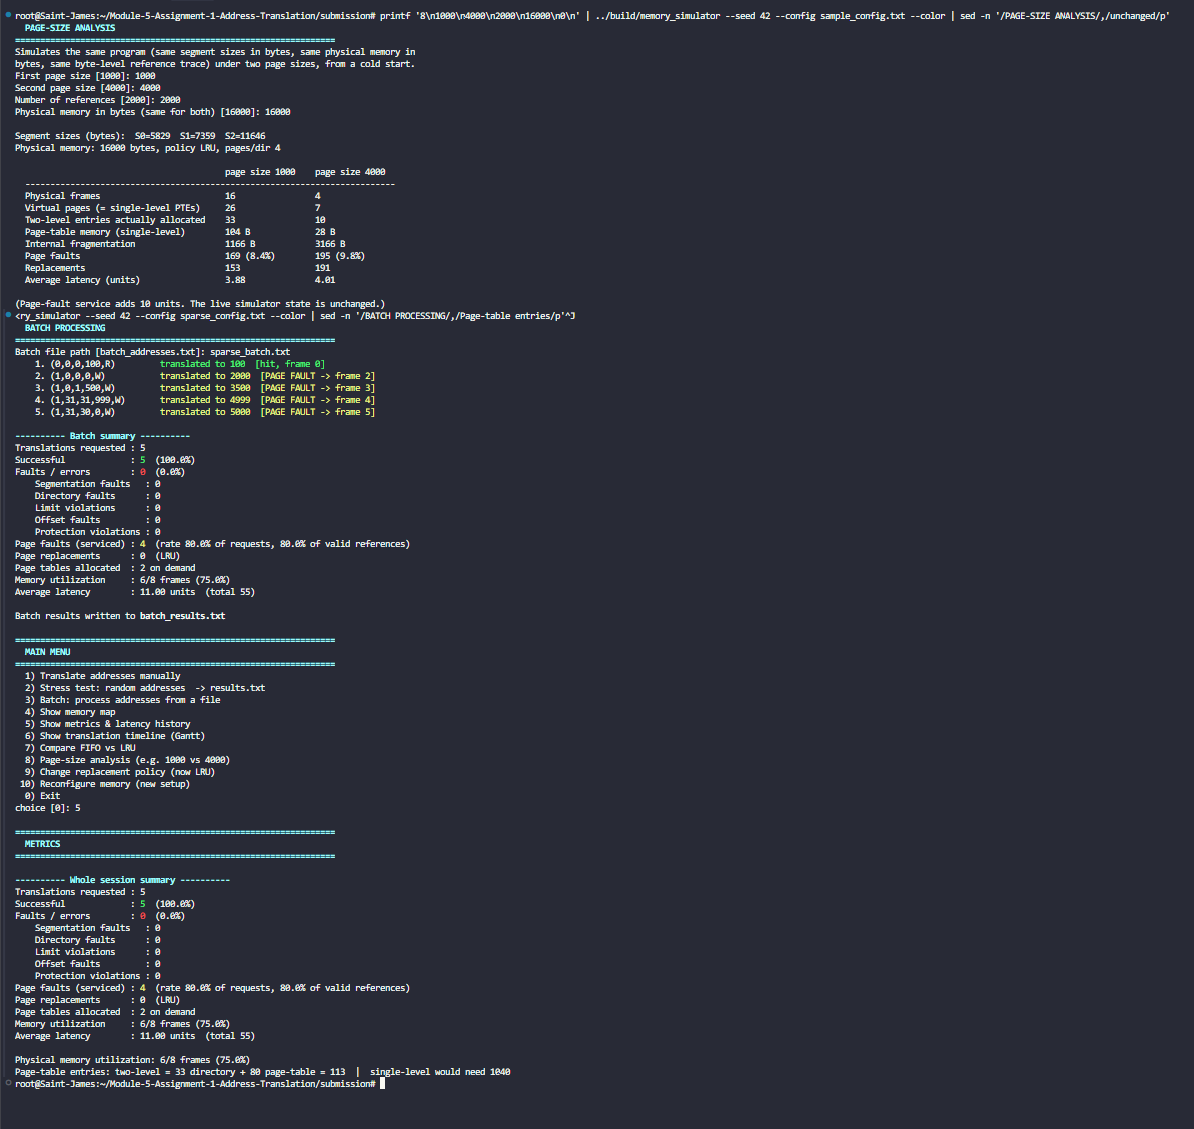
\includegraphics[width=0.75\linewidth,trim={0 252 334.5 161},clip]{11_two_level.png}\\[2pt]
    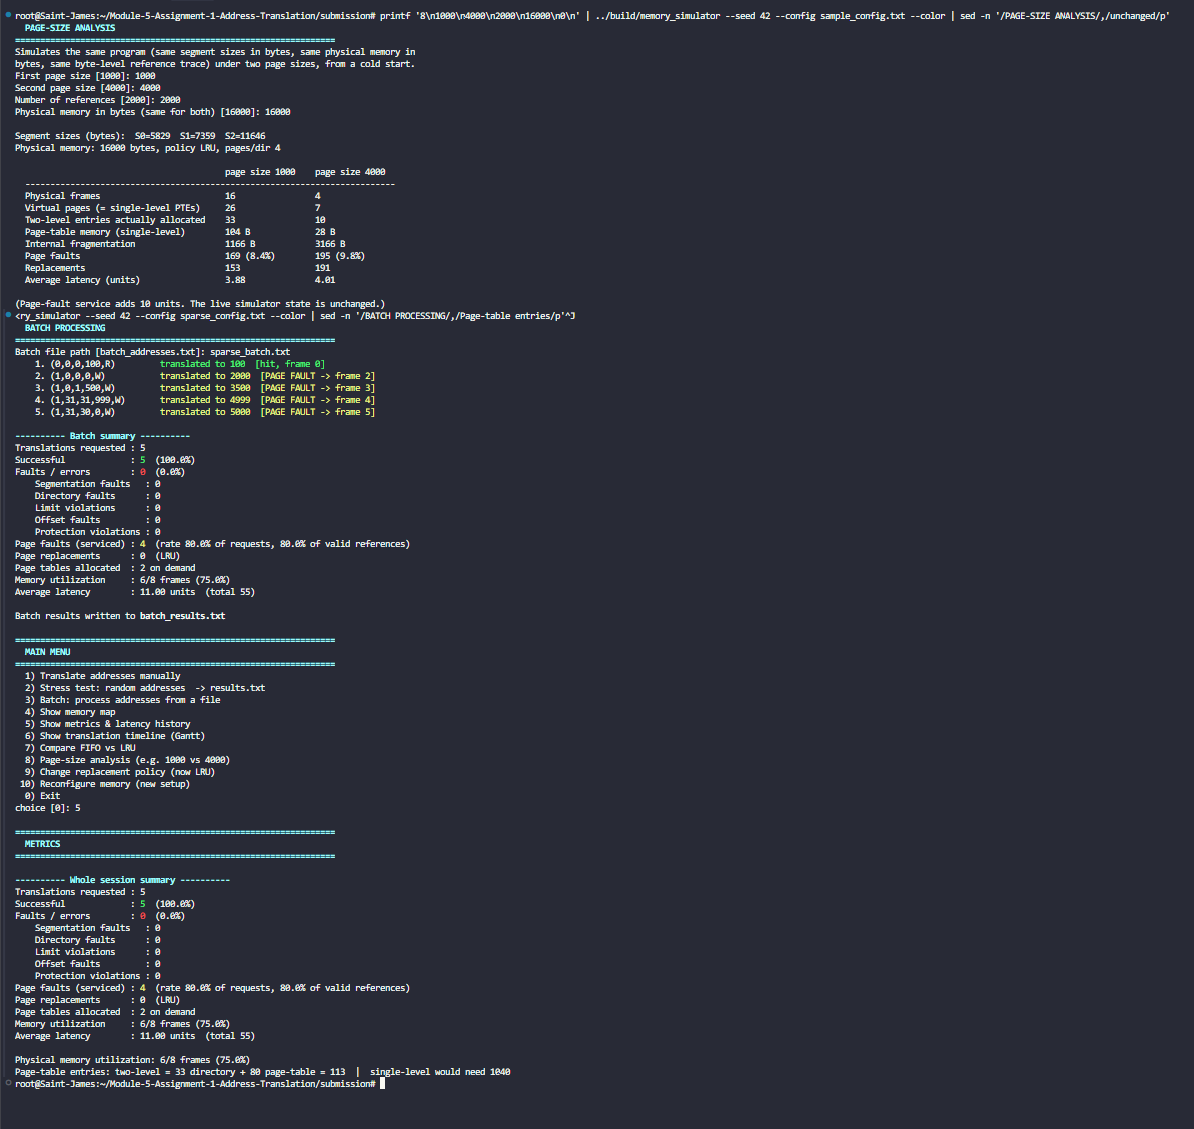
\includegraphics[width=0.75\linewidth,trim={0 24.5 334.5 524},clip]{11_two_level.png}%
  }{%
    \fbox{\parbox[c][3.5cm][c]{0.9\linewidth}{\centering
      \textbf{Screenshot not added yet}\\[4pt]
      save it as \texttt{report/screenshots/11\_two\_level.png}}}%
  }
  \caption{Sparse segment: batch run (top) and the page-table entry count, two-level vs.\ single-level (bottom).}
  \label{fig:twolevel}
\end{figure}

% =============================================================================
\section{Short-Answer Questions}

\question{1. What is the role of the \code{present} bit in the page table, and how does it trigger a page fault?}
The present bit records whether a page is resident in a physical frame. When a legal access
finds it set to 0, \code{getFrameNumber} returns \emph{not present}. The handler then raises a page fault,
loads the page into a free or victim frame, sets the bit to 1 and completes the access.

\question{2. How does a protection violation differ from a segmentation fault?}
A segmentation fault means the address itself is invalid: no such segment, or the address is
outside its limit. A protection violation means the address is valid but the access type is
forbidden, for example writing to a read-only segment or page.

\question{3. Why is a two-level page table useful for large address spaces?}
Only the small directory must be fully allocated. Second-level tables are created only for
regions that are actually used, so a sparse address space needs far fewer entries. In the
sparse test this was 113 entries instead of 1040.

\question{4. Explain the purpose of the \code{base_address} in the segment table.}
The base address tells the translator where the segment's page directory starts in physical memory,
like a per-segment page-table base register. Together with the limit, it defines the segment. In pure
segmentation, the base is instead the start of the segment, and the offset is added to it.

\question{5. How does changing the page size affect the number of page table entries and offset range?}
A larger page size means fewer entries ($\lceil \text{size}/\text{page size}\rceil$) and a wider
offset range ($0 \ldots \text{page size}-1$, i.e.\ more offset bits). A smaller page size means more entries and a
narrower offset range. In the test, 26 entries at 1000 B dropped to 7 entries at 4000 B.

\question{6. What is the main advantage of FIFO over LRU for page replacement?}
FIFO is simpler and cheaper. It only updates a queue when a page is loaded. LRU must record every reference
and search for (or maintain an order of) the least recently used frame.

\question{7. Why might a read-only segment be used in a real OS?}
Read-only segments protect code and constant data from accidental or malicious modification,
such as bugs or code injection. They also let many processes safely share one physical copy of a program or
library.

% =============================================================================
\section{Long-Answer Questions}

\question{8. Describe how the segment table and page table work together to translate a logical address. Use an example from your simulator with specific values.}
Translation is a chain of lookups. Each level narrows the search and adds a check. The segment
table is consulted first. The segment number selects an entry that holds the base address of the
segment's page directory, its limit in pages and its protection. The directory index then selects a
directory entry, which points to a second-level page table. Inside that table, the page number selects a
page-table entry with a frame number, a present bit and page-level protection. Finally, the
offset is appended within the frame: $\textit{physical} = \textit{frame}\times\textit{page size} + \textit{offset}$.

Take translation \#1 from Figure~\ref{fig:manual}, the logical address (1, 0, 2, 250, Read).
Segment~1 exists (valid range 0--2). Its entry says the page directory is at \code{0x2000}, the
limit is 8 pages and the protection is read-write. Directory index~0 is inside the two-entry
directory ($\lceil 8/4\rceil = 2$) and points to an allocated 4-entry page table. Page~2 is below
4 and corresponds to virtual page $0\times4+2 = 2$, within the limit. The offset 250 is below the page
size of 1000. A read is allowed. The entry for page~2 has present = 1 and frame~6, so the result is
$6\times1000+250 = \mathbf{6250}$, with a simulated latency of 3 units.

Other examples show what happens when a lookup cannot finish normally. For (2, 1, 2, 40, Write) the
segment-level checks pass, but directory entry~1 of segment~2 is empty. The simulator first
allocates a page table for that region. The page's present bit is 0, so a page fault is raised. Frame~4 is
still free, so the page is loaded there and the address becomes 4040. The latency is $2 + 10$ units, because
the fault-service penalty is added. For (1, 1, 3, 100, Read), virtual page $1\times4+3 = 7$
is not resident and all 7 frames are in use. LRU chooses the frame with the oldest last use,
frame~0 (owned by S1:D0:P0). It clears that page's present bit, loads page~7 into frame~0 and
returns physical address 100. Each level validates its part of the address first: the segment
table checks existence, limit and segment rights, and the page table checks presence and page rights.
This is why every error can be reported precisely, for example ``Invalid segment 5, max 2''.

\question{9. Explain the trade-offs of FIFO vs.\ LRU page replacement in the context of your simulator. Which performs better for random workloads, and why?}
In the simulator, FIFO uses a queue of frames in load order. A page fault evicts the front of the
queue, and the reloaded frame moves to the back. LRU stores a last-use time per frame. This value
is updated on \emph{every} successful reference, and a fault scans the frames for the minimum. So
FIFO's cost is paid only on faults, while LRU's bookkeeping is paid on every access, plus an
$O(\text{frames})$ search per fault. Real hardware can rarely afford exact LRU, which is why
approximations such as the clock algorithm exist. FIFO can also show Bélády's anomaly, where more frames
cause more faults. LRU is a stack algorithm and cannot.

The comparison experiment (Figure~\ref{fig:fifolru}) replays the same reference strings from the
same memory state under both policies. With a \emph{uniform random} workload, FIFO had 733 faults
and LRU 732 out of 1000. That is effectively a tie, and it is what theory predicts: when every page is
equally likely next, recency carries no information. Any policy that keeps some 7 of the 26
pages has about the same hit chance ($7/26 \approx 27\%$, i.e.\ about a 73\% fault rate). For random
workloads, then, neither policy wins. FIFO is the better engineering choice there because it gives the
same result for less work.

The picture changes once the workload has structure. With 80/20 locality (80\% of references go
to a 5-page hot set), LRU had 216 faults against FIFO's 306, about 29\% fewer. LRU keeps the hot pages
because they are always recently used. FIFO evicts them as soon as they reach the head of the queue,
however often they are used. The third workload loops over 8 pages with only 7 frames. This is LRU's
worst case: the page it evicts is always the one needed next, so it faulted on 998 of 1000
references. FIFO faulted on 502, because the loop and the queue drift out of phase. The conclusion
is that LRU is better for typical programs, which have locality, FIFO is as good for random access, and
cyclic access patterns larger than memory defeat LRU.

\question{10. Discuss the challenges of implementing protection checks in your simulator. How do they improve system security, and what are the potential performance costs?}
The first challenge was \emph{where} the checks belong. Protection exists at two levels. A segment
can be read-only as a whole (the code segment), and individual pages inside a read-write segment can
also be read-only (page~3 of segment~1). The simulator checks the segment first and then the page
entry. A page cannot be more permissive than its segment, so the config loader forces pages of a
read-only segment to read-only.

The second challenge was \emph{ordering}, and the starter code shows why it matters. The
starter checked the present bit before protection. On a page fault it then called
\code{setFrame(page, frame, accessType)}, which overwrote the page's protection with the access type.
A write to a non-resident read-only page therefore faulted, the page was loaded \emph{as read-write}
and the write succeeded. That is a privilege escalation caused by a missing check. In the simulator,
protection is a fixed attribute of the page-table entry, independent of residency. It is checked
before the fault handler runs, so an illegal write never loads a page or changes memory state. The
stress test shows this works: even at a valid ratio of 1.0, all 16 failures were protection
violations from random writes to read-only regions.

Protection improves security in several ways. It keeps code from being overwritten, which
blocks a whole class of code-injection attacks. It isolates a process's constant data. It also makes
sharing safe: many processes can map one physical copy of a library only if none of them can write it.
Every violation is logged with a reason in \code{errors.log}, which in a real OS corresponds to
delivering a signal such as SIGSEGV and auditing the event.

The cost per translation is small: two comparisons, which in hardware are done in parallel
by the MMU, with the permission bits cached in the TLB beside the frame number. The larger costs are
indirect. Permission bits make TLB entries larger. Changing a page's protection requires a TLB
shootdown on multiprocessor systems. Each violation also traps into the kernel, which costs a context
switch. In the simulator, a rejected access still pays its 1--5 latency units, but it never pays the
10-unit fault penalty, so failing early is also the cheaper path.

\question{11. Analyze the impact of page size on memory efficiency and translation overhead. Use your simulator to illustrate with two different page sizes (e.g., 1000 vs.\ 4000).}
Page size is a trade-off between \emph{page-table overhead} and \emph{internal fragmentation}, and
it also affects how well memory can follow a program's working set. The page-size analysis
(Figure~\ref{fig:pagesize}) runs the same program under both sizes: three segments of 5829, 7359
and 11646 bytes, 16000 bytes of physical memory and the same 2000-reference byte-level trace with
80/20 locality.

\emph{Table overhead.} At 1000 bytes per page, the program needs 26 pages, so a single-level design needs
26 entries (104 bytes). At 4000 bytes it needs only 7 entries (28 bytes), a 3.7$\times$ reduction. The offset
grows from 0--999 to 0--3999. Fewer, larger pages also mean that each TLB entry covers four times as much
memory, so the TLB misses less often and fewer translations need a page walk.

\emph{Internal fragmentation.} Each segment's last page is only partly used. With 1000-byte pages
the waste totals 1166 bytes. With 4000-byte pages it grows to 3166 bytes, almost 20\% of the
16000-byte memory. Large pages waste memory in the last page of every segment.

\emph{Fault behaviour.} The same 16000 bytes provide 16 small frames or only 4 large ones. With
4000-byte pages, each fault brings in more data, which helps sequential access (prefetching). But
memory can hold only 4 distinct regions, so a hot set spread over three segments competes for very
few slots. Small pages let memory hold exactly the hot parts. The result was 169 faults (8.4\%) with
1000-byte pages against 195 (9.8\%) with 4000-byte pages, and average latency rose from 3.88 to 4.01
units. In a real system each large-page fault also transfers four times more data from disk,
which the simulator's flat 10-unit penalty understates.

Larger pages therefore lower translation overhead (smaller tables, better TLB reach), and smaller
pages use memory more efficiently (less fragmentation, finer working sets). Real systems use a
moderate default (4~KB) and offer optional huge pages (2~MB/1~GB) for large, dense regions such as
databases.

\question{12. Explain how multi-level page tables reduce memory usage compared to single-level tables. Provide a scenario where your two-level implementation is beneficial.}
A single-level page table needs one entry for \emph{every} virtual page in the address space,
whether or not the page is ever used. The table is indexed directly by page number, so it must be contiguous
and fully allocated. For a 32-bit space with 4~KB pages that is $2^{20}$ entries (4~MB) per process.
Most processes, however, use only a few compact regions, such as code and heap at the bottom and the stack at the top,
with a huge unused gap between them.

A two-level table splits the page number into a directory index and a page index. The directory is
small and always present. A second-level table is allocated only when some page in its range is used,
and an empty directory entry stands for a whole unused range of pages at the cost of one entry. Memory
use therefore grows with the parts of the address space actually used, not with its total size. The cost is one
extra memory access per translation on a TLB miss.

The simulator implements this in \code{DirectoryTable}. Each directory entry is a
\texttt{std::\allowbreak optional<\allowbreak PageTable>} that stays empty until the first access to its range. That access
appears in the trace as ``entry was empty $\rightarrow$ allocated a new page table''. The memory map
prints unallocated entries as ``(not allocated -- no page table)'', and the metrics compare the two-level
footprint with the single-level equivalent.

A scenario where this helps is \code{sparse_config.txt}, which models a process with a 16-page code segment and
a 1024-page (about 1~MB) data segment for heap and stack, with 32 pages per directory entry. The
program touches only the start of the heap (directory~0) and the top of the stack (directory~31).
Only those two page tables are created. The total is $33$ directory entries $+ 80$ page-table entries
$= 113$, compared with 1040 for a single-level table. That is 452 bytes instead of 4160 bytes, 89\% less
(Figure~\ref{fig:twolevel}). The saving grows with sparseness: if the stack later grows downward,
only the directories it reaches are allocated.

For small, dense segments, two levels can cost slightly \emph{more}. In the sample configuration, the
two-level total was 27--33 entries against 26 for a single-level table, because the directory entries are overhead. Multi-level
tables pay off for large, sparse address spaces, which is the common case in real systems.

\question{13. Describe how your simulator handles dynamic memory configuration. Discuss challenges in ensuring valid configurations (e.g., preventing over-allocation).}
The configuration can be set three ways. (1) At start-up, interactive prompts ask for the number of
frames, page size, number of segments, pages per directory entry and replacement policy. Each
prompt shows a default and re-asks on invalid input, for example ``Please enter a whole number from 1 to 4096''.
Segments are then created randomly: limits of 4--12 pages, about a quarter read-only, some directory
entries left empty and about 40\% of pages resident in random free frames. (2) A configuration file
(\code{--config} or the start-up prompt) gives exact control. Each segment line lists its ID, base,
limit, protection and per-page tokens such as \code{6:RW} or \code{-:RO}. (3) The \emph{Reconfigure}
menu item rebuilds memory at runtime without restarting the program. The policy can also be switched at
any time.

Validation happens at several layers. Each value is range-checked: frames 1--4096, page size up to 1\,000\,000, at most
32 segments, limits 1--4096 pages. Derived quantities are checked too: frames $\times$ page size must fit in
the address range, otherwise physical addresses would overflow. Structural rules are enforced:
segment IDs must be sequential, because the segment number indexes the table directly. A segment
cannot list more pages than its limit. Page directories may not overlap in memory, a read-only segment
cannot contain writable pages, and frame numbers must exist. The file loader collects \emph{all}
errors with line numbers and rejects the whole configuration, so a half-loaded state can never exist.

Over-allocation was the subtlest challenge, because two different conditions both look like ``too many pages''.
Having more \emph{virtual} pages than frames is legal; that is the purpose of virtual memory. The
sample configuration has 26 pages over 7 frames, and the simulator reports this as a note (``3.71$\times$
over-committed, demand paging will be used''), not an error. What must never happen is more
\emph{resident} pages than frames, or two pages sharing one frame. The starter's random
\texttt{rand() \% 100} frame numbers broke this invariant. The simulator prevents it in three ways: frames are only taken
through \code{claimFrame}, which refuses frames that are in use or out of range; a duplicate frame in a config file is
rejected with the name of the page that already owns it; and \code{validateConfiguration()} checks after start-up that
each resident page maps to a distinct, valid frame whose owner record points back to that page.

\question{14. Evaluate the effectiveness of your stress testing approach. How does varying the valid/invalid address ratio reveal system limitations?}
The stress test generates $N$ addresses (default 100). With probability $r$ (the valid ratio) an address is \emph{in range}:
a random existing segment, a virtual page below the limit, split into directory and page, and a
legal offset. Otherwise one field is deliberately broken (a non-existent segment, an out-of-range
directory, a page past the limit or an offset past the page size), so every error path is exercised.
Access type is random, so in-range addresses can still be protection violations. Every result goes to
\code{results.txt} with its time slot, and every fault reason goes to \code{errors.log}. With a fixed
seed, runs can be reproduced exactly, which allowed the following sweep (seed 42, sample
configuration, 100 addresses):

\begin{center}
\begin{tabular}{@{}crrrr@{}}
\toprule
Valid ratio & Successful & Errors & Page faults & Avg latency \\
\midrule
0.0 & 0 & 100 & 0 & 3.09 \\
0.3 & 22 & 78 & 19 & 5.06 \\
0.5 & 34 & 66 & 29 & 6.01 \\
0.7 & 58 & 42 & 41 & 7.18 \\
0.9 & 71 & 29 & 56 & 8.56 \\
1.0 & 84 & 16 & 58 & 8.89 \\
\bottomrule
\end{tabular}
\end{center}

The sweep shows several things. At $r = 0$, every request is rejected during validation, before any memory
state changes. Latency stays at the bare 1--5 unit range (mean 3.09), which confirms that invalid
addresses are cheap and cannot cause page faults or evictions. As $r$ rises, latency increases almost
in step with the page faults, because each fault adds 10 units. The real bottleneck of the system is
therefore the 7-frame memory, not the checking logic. At $r = 1.0$, 58 of 84 successful references
faulted (69\%). This is consistent with uniform random access to 26 pages through 7 frames and shows that the
configuration thrashes once the working set exceeds memory. Even at $r = 1.0$, 16 requests fail, all of them
protection violations. This shows that ``in range'' is not the same as ``allowed'', and that the
protection logic still works under load.

The approach has limits. Uniformly random addresses have no locality, so they show the worst case for
paging and cannot tell FIFO and LRU apart. The dedicated locality and loop workloads in the FIFO/LRU
experiment address this. Also, only one field is broken per invalid address, so combined errors
test only the first check that fails. Better coverage would replay real program traces, mix in a
skewed (Zipf) distribution, and sweep the frame count to find the point where the fault rate
drops sharply.

\question{15. Propose a real-world application (e.g., embedded system, cloud server) for your simulator. How would you extend it to handle specific requirements (e.g., real-time constraints, multi-threading)?}
One application is a \emph{capacity-planning tool for a multi-tenant cloud server}. A hosting
provider must decide how much RAM to give each virtual machine or container, which page size to use,
and how far memory can be over-committed before tenants start thrashing. The simulator already
models the key mechanisms: protection between regions, demand paging, replacement, utilization and latency
metrics. It also reads configurations from files, so an operator could load real memory layouts and
replay recorded address traces, then compare policies and page sizes before changing production
settings.

Several extensions would be needed for this use.
\begin{itemize}
  \item \textbf{Multiple address spaces.} Today there is one segment table. A server needs one per
        tenant (process), sharing a single \code{PhysicalMemory}. Frames would gain an owner
        process ID, and a TLB with address-space identifiers (ASIDs) would avoid flushing on every
        context switch. Shared read-only segments (libraries) would map the same frames into
        several tables, using the existing protection checks.
  \item \textbf{Multi-threading.} Tenants run concurrently, so translation must be thread-safe. The
        simple approach is a mutex around the frame pool and per-address-space locks on page tables.
        A better approach is a lock-free read path for TLB/page-table hits, with locks only on page faults
        and evictions, plus TLB-shootdown simulation when a page is evicted.
  \item \textbf{Better replacement and quotas.} Add the clock (second-chance) algorithm, dirty bits
        with write-back cost, per-tenant frame quotas and working-set tracking, so that one tenant cannot
        evict everyone else's pages.
  \item \textbf{Realistic costs.} Replace the flat penalty with a model of DRAM, SSD and network-storage latency,
        and report tail latency (99th percentile), not only the mean.
\end{itemize}

The same design could serve an \emph{embedded real-time} controller, such as an automotive ECU, with
different extensions. Real-time code cannot tolerate unbounded page-fault delays, so the extension would add
\emph{page locking} (pinned frames that are never chosen as victims) for time-critical tasks. The simulator's
latency model would also be used to prove a worst-case translation time: each task's deadline would be checked
against the timeline, and the run would be flagged if any translation exceeded its budget. Memory protection would
isolate safety-critical tasks from less trusted ones, which is the role of the MPU on microcontrollers.

% =============================================================================
\section{Challenges and Enhancements}

\paragraph{Challenges.}
\begin{itemize}
  \item \textbf{Eviction needs a reverse mapping.} Replacement picks a \emph{frame}, but it must clear
        the present bit of the \emph{page} that owns it. Each frame therefore records its owner
        (segment, directory, page), and a consistency check confirms that owners and page tables agree.
  \item \textbf{Fixing the starter's protection hole and double relocation} (Section~1.3) required
        separating protection from residency and changing what the base address means.
  \item \textbf{Fair policy comparison.} Comparing FIFO and LRU on different random runs proves
        nothing. The comparison copies the whole simulator state and replays an identical reference
        string under each policy.
  \item \textbf{Reproducibility for the report.} All randomness comes from one seeded
        \code{std::mt19937}, so \code{--seed 42} reproduces every number above.
\end{itemize}

\paragraph{Enhancements beyond the requirements.}
Step-by-step translation traces, colored output, input that accepts commas and parentheses, input echo for
piped sessions, latency history across runs (\code{latency_history.csv}), the FIFO vs LRU and page-size
experiments, sparse-segment demonstration, and a configuration file format with line-numbered errors.

% =============================================================================
\section*{References}
\addcontentsline{toc}{section}{References}
\begin{enumerate}[label={[\arabic*]}]
  \item R.~H. Arpaci-Dusseau and A.~C. Arpaci-Dusseau, \emph{Operating Systems: Three Easy Pieces},
        Arpaci-Dusseau Books, 2018. Chapters 16 (Segmentation), 18--20 (Paging, TLBs, Smaller Tables),
        21--22 (Swapping: Mechanisms and Policies). \url{https://pages.cs.wisc.edu/~remzi/OSTEP/}
  \item A.~Silberschatz, P.~B. Galvin and G.~Gagne, \emph{Operating System Concepts}, 10th ed.,
        Wiley, 2018. Chapters 9 (Main Memory) and 10 (Virtual Memory).
  \item A.~S. Tanenbaum and H.~Bos, \emph{Modern Operating Systems}, 4th ed., Pearson, 2014.
        Chapter 3 (Memory Management).
  \item L.~A. Bélády, ``A study of replacement algorithms for a virtual-storage computer,''
        \emph{IBM Systems Journal}, vol.~5, no.~2, pp.~78--101, 1966.
  \item cppreference.com, C++ standard library reference (\code{std::optional}, \code{std::mt19937},
        \code{std::deque}). \url{https://en.cppreference.com}
\end{enumerate}

\ifincludecode
\appendix
\section{Source Code}
\lstinputlisting[language=C++]{../submission/memory_simulator.cpp}
\fi

\end{document}
